\documentclass[14pt,a4paper,report]{report}
\usepackage[a4paper, mag=1000, left=2.5cm, right=1cm, top=2cm, bottom=2cm, headsep=0.7cm, footskip=1cm]{geometry}
\usepackage[utf8]{inputenc}
\usepackage[english,russian]{babel}
\usepackage{indentfirst}
\usepackage[dvipsnames]{xcolor}
\usepackage[colorlinks]{hyperref}
\usepackage{listings} 
\usepackage{fancyhdr}
\usepackage{caption}
\usepackage{amsmath}
\usepackage{latexsym}
\usepackage{graphicx}
\usepackage{amsmath}
\usepackage{booktabs}
\usepackage{array}
\hypersetup{
	colorlinks = true,
	linkcolor  = black
}

\usepackage{titlesec}
\titleformat{\chapter}
{\Large\bfseries} % format
{}                % label
{0pt}             % sep
{\huge}           % before-code


\DeclareCaptionFont{white}{\color{white}} 

% Listing description
\usepackage{listings} 
\DeclareCaptionFormat{listing}{\colorbox{gray}{\parbox{\textwidth}{#1#2#3}}}
\captionsetup[lstlisting]{format=listing,labelfont=white,textfont=white}
\lstset{ 
	% Listing settings
	inputencoding = utf8,			
	extendedchars = \true, 
	keepspaces = true, 			  	 % Поддержка кириллицы и пробелов в комментариях
	language = Matlab,            	 	 % Язык программирования (для подсветки)
	basicstyle = \small\sffamily, 	 % Размер и начертание шрифта для подсветки кода
	numbers = left,               	 % Где поставить нумерацию строк (слева\справа)
	numberstyle = \tiny,          	 % Размер шрифта для номеров строк
	stepnumber = 1,               	 % Размер шага между двумя номерами строк
	numbersep = 5pt,              	 % Как далеко отстоят номера строк от подсвечиваемого кода
	backgroundcolor = \color{white}, % Цвет фона подсветки - используем \usepackage{color}
	showspaces = false,           	 % Показывать или нет пробелы специальными отступами
	showstringspaces = false,    	 % Показывать или нет пробелы в строках
	showtabs = false,           	 % Показывать или нет табуляцию в строках
	frame = single,              	 % Рисовать рамку вокруг кода
	tabsize = 2,                  	 % Размер табуляции по умолчанию равен 2 пробелам
	captionpos = t,             	 % Позиция заголовка вверху [t] или внизу [b] 
	breaklines = true,           	 % Автоматически переносить строки (да\нет)
	breakatwhitespace = false,   	 % Переносить строки только если есть пробел
	escapeinside = {\%*}{*)}      	 % Если нужно добавить комментарии в коде
}

\begin{document}

\def\contentsname{Содержание}

% Titlepage
\begin{titlepage}
	\begin{center}
		\textsc{Санкт-Петербургский Политехнический 
			Университет Петра Великого\\[5mm]
			Кафедра компьютерных систем и программных технологий}
		
		\vfill
		
		\textbf{Отчёт по лабораторной работе №2\\[3mm]
			Курс: «Методы оптимизации и принятия решений»\\[3mm]
			Тема: «Марковские модели принятия решений»\\[35mm]
			}
	\end{center}
	
	\hfill
	\begin{minipage}{.5\textwidth}
		Выполнил студент:\\[2mm] 
		Бояркин Никита Сергеевич\\
		Группа: 13541/3\\[5mm]
		
		Проверил:\\[2mm] 
		Сиднев Александр Георгиевич
	\end{minipage}
	\vfill
	\begin{center}
		Санкт-Петербург\\ \the\year\ г.
	\end{center}
\end{titlepage}

% Contents
\tableofcontents
\clearpage

\chapter{Лабораторная работа №2}

\section{Индивидуальное задание}

\subsubsection{Вариант 16}

Ежедневно утром производится проверка дорогостоящей машины с целью выявления, находится ли она в исправном состоянии, требует мелкого ремонта или нуждается в серьезном ремонте. Обозначим эти состояния 0, 1, 2 соответственно. Если машина находится в совершенно исправном состоянии, то вероятность того, что она останется в таком же состоянии на начало следующего дня, равна р(0|0), вероятность того, что потребуется мелкий ремонт, равна р(1|0) и вероятность того, что возникает необходимость серьезного ремонта, равна р(2|0). В случае когда машина требует ремонта, фирма может прибегнуть к услугам двух ремонтных фирм, одна из которых (фирма F, гарантирующая качество ремонта) взимает плату М за мелкий ремонт и плату R за крупный. Вторая (фирма Т, не гарантирующая качества ремонта) взымает соответственно плату m и r, где m<М и r<R. Легко себе представить, что качество работ, производимых фирмой F, выше, чем у фирмы Т, что отражается значением вероятности полностью исправного состояния машины на начало следующего за ремонтом дня. Пусть решение d=1 определяет выбор фирмы F и решение d=2 — выбор фирмы Т. Обозначим через р(j | i, d) вероятность перехода машины в состояние j на следующем отрезке (j=0,1,2) при условии, что она находится в состоянии I на текущем отрезке (i=1,2) и принимается решение d(d=1,2).
\\\\
р (0 | 0) = 0.6 (машина осталась исправной)\\
р (1 | 0) = 0.3 (машина требует мелкого ремонта)\\
р (2 | 0) = 0.1 (машина требует крупного ремонта)\\\\
р (0 | 1, 1) = 0.9 [М = 14] (фирма F выполнила мелкий ремонт)\\
р (1 | 1, 1) = 0.1 (фирма F в процессе выполнения мелкого ремонта)\\
р (2 | 1, 1) = 0 (невозможное событие -- если выполнен крупный ремонт, то мелкий не нужен)\\
р (0 | 2, 1) = 0.6 [R = 21] (фирма F выполнила крупный ремонт)\\
р (1 | 2, 1) = 0.3 [R – M = 7] (фирма F выполнила мелкий ремонт, но надо доделать до крупного)\\
р (2 | 2, 1) = 0.1 (фирма F в процессе выполнения крупного ремонта)\\\\
р (0 | 1, 2) = 0.7 [m = 12] (фирма T выполнила мелкий ремонт)\\
р (1 | 1, 2) = 0.2 (фирма T в процессе выполнения мелкого ремонта)\\
р (2 | 1, 2) = 0 (невозможное событие -- если выполнен крупный ремонт, то мелкий не нужен)\\
р (0 | 2, 2) = 0.5 [r = 19] (фирма T выполнила крупный ремонт)\\
р (1 | 2, 2) = 0.4 [r – m = 7] (фирма T выполнила мелкий ремонт, но надо доделать до крупного)\\
р (2 | 2, 2) = 0.1 (фирма T в процессе выполнения крупного ремонта)\\
\\
Найдите оптимальную стратегию и минимальные затраты на отрезке N=$\infty$.

\section{Ход работы}

\subsection{Решения и стратегии}

Имеется три состояния машины:

\begin{itemize}
	\item 1 -- исправна;
	\item 2 -- легкая поломка (необходим мелкий ремонт);
	\item 3 -- серьезная поломка (необходим крупный ремонт);
\end{itemize}

Для данных состояний имеется три решения:

\begin{itemize}
	\item $X_1$ -- ничего не делать;
	\item $X_2$ -- выбрать фирму F;
	\item $X_3$ -- выбрать фирму T;
\end{itemize}

Таким образом, возможны следующие стратегии:

\begin{table}[h!]
	\centering
	\bgroup
	\def\arraystretch{1}
	\begin{tabular}{ | m{0.3cm} | m{2.2cm} | m{2.8cm} | m{3.1cm} | }
		\hline
		№ & Исправна & Легкая поломка & Серьезная поломка \\ \hline
		1 & $X_1, (-)$ & $X_2, (F)$ & $X_3, (T)$ \\ \hline
		2 & $X_1, (-)$ & $X_2, (F)$ & $X_2, (F)$ \\ \hline
		3 & $X_1, (-)$ & $X_3, (T)$ & $X_3, (T)$ \\ \hline
		4 & $X_1, (-)$ & $X_3, (T)$ & $X_1, (F)$ \\
		\hline
	\end{tabular}
	\egroup
\end{table}

\subsection{Построение матриц переходных вероятностей и матриц расходов}

$P_1$ и $P_2$ -- матрицы переходных вероятностей для компаний $F$ и $T$ соответственно:
\\

$
P_1=\begin{bmatrix}
0.6 & 0.3 & 0.1 \\
- & - & - \\
- & - & - \\
\end{bmatrix}
$
$
P_2=\begin{bmatrix}
- & - & - \\
0.9 & 0.1 & 0 \\
0.6 & 0.3 & 0.1 \\
\end{bmatrix}
$
$
P_3=\begin{bmatrix}
- & - & - \\
0.7 & 0.2 & 0.1 \\
0.5 & 0.4 & 0.1 \\
\end{bmatrix}
$\\

$R_1$ и $R_2$ -- матрицы расходов для компаний $F$ и $T$ соответственно:
\\

$
R_1=\begin{bmatrix}
0 & 0 & 0 \\
- & - & - \\
- & - & - \\
\end{bmatrix}
$
$
R_2=\begin{bmatrix}
- & - & - \\
14 & 0 & 0 \\
21 & 7 & 0 \\
\end{bmatrix}
$
$
R_3=\begin{bmatrix}
- & - & - \\
12 & 0 & 0 \\
19 & 7 & 0 \\
\end{bmatrix}
$\\

\subsection{Нахождение величин ожидаемого дохода}

Ожидаемый доход вычисляется по формуле:\\

$\nu_i(X_{k})=\sum_{j=1}^{m}p_{i,j}(X_{k})r_{i,j}(X_{k})$\\

Тогда для первого решения (ничего не делать):\\

$\nu_1(X_1)=0$

$\nu_2(X_1)=-$

$\nu_3(X_1)=-$\\

Для второго решения (выбрать фирму F):\\

$\nu_1(X_2)=-$

$\nu_2(X_2)=0.9\cdot 14=12.6$

$\nu_3(X_2)=0.6\cdot 21+0.3\cdot 7=14.7$\\

Тогда для третьего решения (выбрать фирму T):\\

$\nu_1(X_3)=-$

$\nu_2(X_3)=0.7\cdot 12=8.4$

$\nu_3(X_3)=0.5\cdot 19+0.4\cdot 7=12.3$\\

\clearpage

\subsection{Формулировка задачи в виде задачи линейного программирования}

Приведение к задаче линейного программирования производится следующим образом:

\begin{figure}[h!]
	\centering
	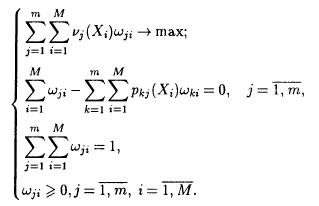
\includegraphics[scale = 0.90]{images/1.png}
	\label{image:1}
\end{figure}

Для данной задачи:

\begin{equation*}
	\begin{cases}
		\text{$0\cdot w_{11}+12.6\cdot w_{22}+8.4\cdot w_{23}+14.7\cdot w_{32}+12.3\cdot w_{33}\rightarrow min$} \\
		\text{$(1-0.6)\cdot w_{11}-0.9\cdot w_{22}-0.7\cdot w_{23}-0.6\cdot w_{32}-0.5\cdot w_{33}=0$} \\
		\text{$-0.3\cdot w_{11}+(1-0.1)\cdot w_{22}+(1-0.2)\cdot w_{23}-0.3\cdot w_{32}-0.4\cdot w_{33}=0$} \\
		\text{$-0.1\cdot w_{11}-0\cdot w_{22}-0.1\cdot w_{23}+(1-0.1)\cdot w_{32}+(1-0.1)\cdot w_{33}=0$} \\
		\text{$w_{11}+w_{22}+w_{23}+w_{32}+w_{33}=1$}
		\text{$w_{ij}\geq 0, i=\overline{1,2,3}, j=\overline{1,2,3}$}
	\end{cases}
\end{equation*}

\subsection{Решение задачи}

Разработаем скрипт для расчета вероятностей $w_{ij}$ в среде MATLAB:

\lstinputlisting{listings/l1.m}

Результат расчета вероятностей:

\lstinputlisting{listings/l1.log}

Таким образом машина исправна с вероятностью 61.82\%. Для мелкого ремонта следует обращаться в фирму T (28.18\%). Для крупного ремонта следует обращаться в фирму F (10\%).

\subsection{Дополнительное задание}

Предположите, что фирме F для выполнения крупного ремонта требуется 1 полный рабочий день, а фирме Т — 2 полных рабочих
дня. Считайте далее, что фирма — владелец машины несет потери в размере $c$ единиц за каждый день ее простоя. Покажите, как при этих условиях нужно изменить уравнения.

Для решения задачи нет смысла определять новые состояния, как это указано в методических указаниях. Достаточно просто изменить матрицы расходов для компаний $F$ и $T$ следующим образом:\\

$
R_1=\begin{bmatrix}
0 & 0 & 0 \\
- & - & - \\
- & - & - \\
\end{bmatrix}
$
$
R_2=\begin{bmatrix}
- & - & - \\
14 & 0 & 0 \\
21 + c & 7 + c & 0 \\
\end{bmatrix}
$
$
R_3=\begin{bmatrix}
- & - & - \\
12 & 0 & 0 \\
19 + 2\cdot c & 7 + 2\cdot c & 0 \\
\end{bmatrix}
$\\

Дальше задача решается аналогичным образом.

\section{Вывод}

В ходе данной лабораторной работы были определены оптимальные стратегии для конкретной задачи. Машина исправна с вероятностью 61.82\%. Для мелкого ремонта следует обращаться в фирму T (28.18\%). Для крупного ремонта следует обращаться в фирму F (10\%).

Линейное программирование позволяет достаточно легко и быстро решать подобные задачи.

\end{document}